% ============================================================
%  项目报告 —— 日语歌词汉译配的音节约束与文本质量评估
%  编译：xelatex main.tex -> bibtex main -> xelatex main.tex -> xelatex main.tex
%        或 latexmk -xelatex main.tex
%  说明：正文基于 1th.docx；第三章按“任务难点—技术路线—三项设计”重写。
%        封面信息（姓名/学号等）仍需自行填写。
% ============================================================
\documentclass[12pt, a4paper]{ctexart}

% ---------- 页面与版式 ----------
\usepackage[margin=2.5cm]{geometry}
\usepackage{setspace}
\onehalfspacing

% ---------- 常用宏包 ----------
\usepackage{amsmath, amssymb, amsthm}
\usepackage{graphicx}
\usepackage{float}
\usepackage{booktabs}      % 三线表
\usepackage{multirow}
\usepackage{array}
\usepackage{longtable}
\usepackage{threeparttable}
\usepackage{caption}
\usepackage{subcaption}
\usepackage{enumitem}
\usepackage{xcolor}
\usepackage{hyperref}
\usepackage{url}
\usepackage{listings}      % 代码块
\usepackage{algorithm}
\usepackage{algpseudocode}
\usepackage{fancyhdr}
\usepackage{titlesec}

% ---------- 章节编号：一、 / （一） / 1. ----------
\ctexset{
  section/name           = {,、},
  section/number         = \chinese{section},
  subsection/name        = {（,）},
  subsection/number      = \chinese{subsection},
  subsubsection/name     = {,.},
  subsubsection/number   = \arabic{subsubsection},
}

% ---------- 图表按节编号（表 4-1、图 4-1 ……） ----------
\numberwithin{table}{section}
\numberwithin{figure}{section}
\renewcommand{\thetable}{\arabic{section}-\arabic{table}}
\renewcommand{\thefigure}{\arabic{section}-\arabic{figure}}

% ---------- 超链接样式 ----------
\hypersetup{
  colorlinks = true,
  linkcolor  = blue!60!black,
  citecolor  = blue!60!black,
  urlcolor   = blue!60!black,
}

% ---------- 代码块样式 ----------
\lstset{
  basicstyle   = \ttfamily\small,
  breaklines   = true,
  frame        = single,
  numbers      = left,
  numberstyle  = \tiny\color{gray},
  keywordstyle = \color{blue!70!black},
  commentstyle = \color{green!50!black},
  stringstyle  = \color{orange!80!black},
  showstringspaces = false,
  captionpos   = b,
}

% ---------- 页眉页脚 ----------
\pagestyle{fancy}
\fancyhf{}
\fancyhead[L]{\small 项目报告}
\fancyhead[R]{\small\leftmark}
\fancyfoot[C]{\thepage}
\renewcommand{\headrulewidth}{0.4pt}

% ---------- 图表标题格式 ----------
\captionsetup{font=small, labelsep=quad}
\captionsetup[table]{skip=4pt}

% ---------- 定理环境（按需保留） ----------
\newtheorem{definition}{定义}[section]
\newtheorem{theorem}{定理}[section]

% ---------- 自定义命令 ----------
\newcommand{\sysname}{workflow-rag}

% ============================================================
\begin{document}

% ---------- 封面信息 ----------
\begin{titlepage}
  \centering
  \vspace*{3cm}
  {\Huge\bfseries 日语歌词汉译配的音节约束与文本质量评估\par}
  \vspace{2.5cm}
  {\large
    \begin{tabular}{rl}
      课程/项目名称： & TODO \\
      姓名：         & TODO \\
      学号：         & TODO \\
      专业/班级：    & TODO \\
      指导教师：     & TODO \\
      完成日期：     & \today \\
    \end{tabular}
  \par}
  \vfill
\end{titlepage}

% ---------- 摘要 ----------
\begin{abstract}
\noindent
日语歌词汉译配需兼顾情绪表达与音节匹配，中文直译偏短及模型计数不准增加了难度。本项目引入人工音节预算和分组标注，结合意境分析、初稿生成、诗歌检索改写与程序校验返修，构建可追溯的译配流程。以论文原提示词、人工标注适配和单次归档 writer 为对照，在 19 首歌曲、380 个有效乐句上开展规则统计与匿名模型评审。人工预算适配使通过率由 12.85\% 升至 39.81\%，完整流程达到 100\%，表现力为 3.91/5，但核心语义保留较弱。无 RAG 流程同样全部达标，RAG 文本偏好胜率为 57.87\%，尚未确认稳定增益。结果说明，程序校验可提高约束执行的可靠性，但译配仍需权衡音节与文本质量，实际可唱性有待真人试唱验证。

\vspace{0.5em}
\noindent\textbf{关键词：}\ 日语歌词汉译配；音节预算；检索增强生成；迭代改写；大模型评价
\end{abstract}

\newpage
\tableofcontents
\newpage

% ============================================================
\section{问题背景与项目目标}
% ============================================================

\subsection{任务背景与应用意义}
歌词译配是受到音乐结构约束的跨语言文本生成任务。与主要服务于内容理解的歌词翻译相比，译配不仅需要传达原歌词的主题，还需要调整目标语言的字句，使其能够配合既有旋律、节拍和乐句结构进行演唱。因此，译配结果的质量不能仅通过语义相似程度衡量，还应综合考虑自然度、节奏适配和表达效果。Štěpánková 和 Rosa~\cite{stepankova-rosa-2025-song} 将可唱译配视为多个目标之间的平衡问题，并尝试将可唱性、意义、自然度、节奏和押韵等要求转化为可分析的评价维度。因此，译配是较难的工作，工作量也较大，往往需要训练有素的专家来完成。如果 AI 能为译配提供参考，将会让更多热爱音乐的普通人也能用母语唱出自己喜爱的歌曲。

\subsection{任务难点}
日语歌词汉译配具有较为突出的音节补足问题。含义相同的一句歌词，日语所使用的音节多于中文，因此直接翻译得到的中文歌词往往长度过短，难以配合旋律演唱。若仅保持直译结果，译词可能无法充分覆盖原曲的节拍；若机械性地增加虚词或使用叠词，又容易破坏自然度和表现力。因此将目标局限于百分百地保留原歌词的含义是行不通的，译配者需要在歌词含义的保真度与歌词的自然度、表现力之间取舍。

\subsection{项目目标与研究问题}
本项目旨在构建一个结合结构化标注、分工生成、外部检索与程序校验的日语歌词汉译配流程，并建立可追溯的实验和评价机制。具体研究问题如下：
\begin{enumerate}[leftmargin=2em]
  \item 人工标注的作用：将目标音节预算和分组信息显式提供给模型，能否提高输出对人工预算的满足程度？
  \item 工作流的作用：通过意境分析、生成和规则反馈组织多阶段处理，能否提高约束执行的可靠性，其文本质量代价是什么？
  \item 检索增强的作用：引入诗歌检索与改写后，是否能够进一步改善情绪表达、自然度和表现力？
\end{enumerate}
围绕上述问题，项目分别记录预算满足情况、文本质量评分和成对偏好，不预设某一种配置在所有维度上均具有优势。

\subsection{研究范围}
本项目研究范围限定为已有歌词文本及结构化标注条件下的日语到中文译配，不涉及基础语言模型的参数训练，也不直接开展音频到歌词、乐谱识别或歌声合成研究。当前系统主要处理歌词原文、目标音节预算、分组参考以及上下文信息。

项目采用的预算由人工整理，其中部分标注包含基于文本发音的估算，尚未统一完成实际演唱校准。日语音拍（mora）数、中文音节数与旋律音符数也不能直接等同。因此，本项目首先验证的是对既定文本预算的执行能力，实际旋律贴合程度仍属于后续需要通过演唱验证的内容。

% ============================================================
\section{已有研究工作}
% ============================================================

\subsection{可唱译配的问题建模与评价}
可唱歌词翻译具有多目标性质。Štěpánková 和 Rosa~\cite{stepankova-rosa-2025-song} 将 Low 的译配“五项原则”进行计算化解释，围绕可唱性、意义、自然度、节奏和押韵建立评价方法，并在英语到捷克语的任务中结合人工译配及人类评价开展分析。这项工作表明，译配质量不能简化为单一的语义准确性或长度匹配问题，而应考察多个目标之间的协调关系。

该研究为本项目提供了评价设计上的启示：音节约束与文本质量应分别报告，不能以一个维度替代其他维度。同时，其语言方向和数据条件与日语汉译配存在差异，相关指标和经验结论仍需要结合目标语言的发音、分词和演唱特点进行适配。

\subsection{约束歌词翻译与质量优化}
长度要求可以在生成的不同阶段介入。Kikuchi 等~\cite{kikuchi-etal-2016-controlling} 在神经摘要任务中将目标长度提供给解码器。对于需要指定词语的机器翻译，Hokamp 和 Liu~\cite{hokamp-liu-2017-lexically} 在搜索时追踪哪些约束已经满足，Post 和 Vilar~\cite{post-vilar-2018-fast} 进一步通过动态分配搜索空间降低开销。本项目通过接口调用生成模型，无法直接控制其解码搜索，因此将音节预算写入输入，再用独立程序校验输出。

Ou 等~\cite{ou-etal-2023-songs} 将歌词翻译建模为受约束的神经机器翻译问题，将长度、押韵及词边界等要求纳入可控制的生成框架，并应用于英语到中文的歌词翻译。作者报告的长度准确率、押韵准确率和词边界召回率分别达到 99.85\%、99.00\% 和 95.52\%。该工作说明，将音乐相关要求转化为显式控制信号能够获得较高的约束满足程度。不过，这些结果建立在其特定训练方法、数据集和评价定义之上，不能与本项目的人工预算通过率直接横向比较。

Ye 等~\cite{ye-etal-2024-sing} 进一步关注约束满足与翻译质量之间的关系，提出结合奖励模型、两阶段训练及推理阶段优化的方法。该研究通过自动评价和人工评价表明，在保持关键可唱性特征的同时，翻译质量仍有进一步优化空间。与仅强调长度或押韵的处理方式相比，这一路线更加重视语义和整曲表达质量，但也需要相应的训练数据与模型优化过程。

上述研究对本项目的启示在于：高约束满足度是译配的重要条件，但不是充分条件。即使系统能够严格满足长度要求，仍需检查情绪、自然度和表达内容是否发生不合理变化。

\subsection{大模型提示词与多模态方法}
Liu 等~\cite{hanze-etal-2026-towards} 针对大语言模型的可唱歌词翻译能力，系统比较了七种提示策略，包括显式核验、多轮修改和利用段落上下文等设置。研究发现，多轮提示能够改善部分节奏与音系相关指标，而提示复杂度与人类感知质量之间并非简单的单调关系。该研究是本项目论文提示词基线的直接来源。本项目选取其中的 Exp.4 指令，并进一步构造提供人工预算与分组信息的适配版本。

需要指出，复用提示词并不等于复现原论文全部实验。原论文与本项目在模型、歌曲样本、计数目标和评价过程上均存在差异。因此，本项目只能通过该基线分析出论文提示策略在当前任务条件下的表现，难以做到对原论文发表成绩的直接重复。

Cho 等~\cite{cho-etal-2025-mavl} 提出 MAVL 多语言音频、视频与歌词数据集，并构建利用音视频信息和音节约束的 SylAVL-CoT 方法。其研究表明，声音与场景信息可以为歌词翻译提供纯文本输入之外的上下文。这一方向提示，真实可唱性还涉及旋律、发声和场景等因素。本项目当前采用文本与预算标注，实施成本较低，但没有直接利用这些多模态信息。

音乐与文本之间的约束还取决于生成方向。Ju 等~\cite{ju-etal-2021-telemelody} 从歌词出发，以包含节奏和终止式等信息的模板引导旋律生成。Tian 等~\cite{tian-etal-2023-unsupervised} 从给定旋律出发，将乐句分段和节奏对齐转化为歌词解码约束。日语歌词汉译配还要保留原词的内容。人工预算只记录旋律对文本长度的部分要求，给定同一预算的两种措辞，其重读位置和演唱难度仍可能不同。

\subsection{检索增强与迭代改写}
Lewis 等~\cite{lewis-etal-2020-rag} 提出的检索增强生成方法，将外部非参数化知识与语言模型生成过程结合，并在知识密集型任务中取得改善。本项目借鉴其“检索材料参与生成”的基本思想，将外部材料用于诗歌意象和语言表达参考。由于诗歌风格改写与事实问答的目标不同，通用 RAG 的实验结论不能直接证明其在歌词译配中的有效性，仍需针对本任务单独检验。

Madaan 等~\cite{madaan-etal-2023-selfrefine} 提出 Self-Refine，通过初次生成、反馈和迭代修改改善模型输出，无需额外训练即可开展推理阶段优化。该方法为本项目的反馈返修机制提供了参考。对于计数等可以确定计算的任务，本项目将反馈来源落实为程序检查，减少对模型自查准确性的依赖；对于意境和表达等开放性目标，则继续由生成模型负责改写。

\subsection{大模型评价及其局限}
Zheng 等~\cite{zheng-etal-2023-judging} 研究了使用大模型评审开放式生成结果的方法，并分析了位置偏差、长度偏差和自我偏好等问题。这类方法能够以较低的人工组织成本提供多维判断和比较依据，但其可靠性取决于评审模型、提示词和任务条件。

本项目据此采用匿名标签、随机展示顺序及交换顺序复评，并要求评分附带具体乐句依据。不过，这些措施只能缓解部分偏差，不能保证评审与人类判断完全一致，尤其无法替代真实演唱条件下的可唱性评价。

在机器翻译任务中，Kocmi 和 Federmann~\cite{kocmi-federmann-2023-large} 比较了有、无参考译文条件下的大模型评分，并在系统层面与人工判断进行对照。Liu 等~\cite{kocmi-federmann-2023-gemba} 使用分维度评价准则指导模型判断生成文本。对于歌词，分别评价语义、意境、自然度和表现力，才能区分同一译句在哪些方面获得认可。Freitag 等~\cite{freitag-etal-2021-experts} 还说明，专业评审、错误类别及篇章上下文会影响人工翻译评价。后续校准宜向双语评审提供上下文，再由试唱者另行评价旋律贴合度。

\subsection{现有研究对本项目的启示}
已有工作分别从约束建模、模型训练、提示词优化、多模态输入及评价方法等方面推进了歌词译配研究。本项目的切入点是面向日语汉译配，在不进行基础模型训练的条件下，将人工预算、意境导向的改写、诗歌检索和确定性校验组织为可追溯的处理流程。

因此，本项目的主要研究价值在于任务适配、流程集成和对照分析：验证模型能否执行人工预算，观察创作性扩展带来的质量取舍，并检验检索改写的额外收益。相关方法来源于已有研究，其组合效果需要由本项目实验具体说明。

% ============================================================
\section{Workflow 模型设计}

本章说明系统如何将保证可唱性的译配任务拆解为可执行的流程。第二章介绍的已有工作大致沿两条路线推进：训练受约束的翻译模型，或在提示词层面不断加约束。前者需要成对训练数据与可控制的解码过程；后者受限于通用模型对“数数”这类精确操作的不稳定。本项目选择第三条路径：不训练模型，而是把译配拆成若干可以分别验证的子任务，交给不同的智能体，并用确定性规则严格约束音节数的匹配。

本章先归纳任务本身的四个技术难点，再给出总体技术路线，然后依次说明三项设计——多智能体 workflow、人工音节预算标注与现代诗检索增强——各自回应哪些难点。

\subsection{任务难点}

第一章已经指出，日语歌词汉译配的核心矛盾是音节补足与语义保真之间的取舍。要把这个矛盾变成可执行的系统，还需要把它拆得更。它可以拆分出下面四个难点：

\newcommand{\subsub}[1]{\phantomsection\subsubsection*{#1}\addcontentsline{toc}{subsubsection}{#1}}

\subsub{难点一：日语与汉语的音节数量难以匹配}

日语的节奏单位是拍（mora），一个假名基本占一拍，助词、活用词尾、敬语成分都要占拍；汉语以字为音节单位，且信息密度大于日语，相同意思的一句话，字数往往明显少于日语的拍数。以一句日文歌词为例，“きっとあなたは何も言わないままで”共 17 拍，而意思最贴近的直译“你一定什么都不说”只有 8 个汉字，中间差出 9 个音节。

音节的差额带来的直接后果是：照原意直译，译词覆盖不住旋律，唱到后半句就只能拖长音或空着；为了凑够拍数而添加“啊”“哦”这类语气词，或者“了”“吧”这种无意义的虚词，又会让歌词冗长不自然。这两种做法都不可取。

\subsub{难点二：模型听不到旋律，可唱的音节数不等于 mora 数}

大模型只接收文本，它不知道这首歌的速度、每个音符的时值、乐句在哪里断，也不知道哪个字会在演唱时被连读、哪个音会被延长。而“一句能唱几个汉字”恰恰由这些信息决定。

更关键的是，可唱的音节数与 mora 数并不是一回事。日语歌会出现快速地连读两个音节的情况，但这在汉语中会很不自然；促音「っ」占一拍却不发声，长音「ー」占一拍但只是延长前一个音节，拗音「きゃ」写作两个假名却只占一拍——因此无论数假名还是数 mora，都换算不出“这句该唱几个汉字”。中文一侧同样有变数：儿化、多音字、轻声都会改变实际唱出的音节。

既然这个量无法从文本推断，就只能由人听着旋律来确定。系统于是把“这句能唱几个汉字”作为人工先验写进数据，自己只负责执行、不负责推断。这是后文第二项设计（人工音节预算标注）的由来。

\subsub{难点三：创作性写作与满足音阶约束是两种相互冲突的任务}

体会情绪意境是创作性的任务，也是发散型的任务，需要联想、越界，把原词没有写出的画面补出来；严格对齐音节是收敛型的任务：需要逐字核对、删减，服从一个外部给定的数字。两者对模型的要求几乎相反——前者希望它“不要太听话”，后者希望它“精确听话”。

把两者压进同一个提示词，模型就会在两种模式之间摇摆：写得放开，字数失控；盯住字数，句子就会不自然且表现力欠缺。Liu 等~\cite{hanze-etal-2026-towards} 也观察到，提示的复杂度与人类感知质量之间并非单调关系，把要求一条条叠上去，并不能同时提升两类指标。这说明问题不在于提示词写得不够长，而在于两类任务本就不该由同一个角色承担。

因此需要把“写”和“对齐”分给不同的智能体，让它们各自使用不同的提示词、不同的采样温度与不同的输出格式；同时把“判定是否达标”从生成过程中独立出来，交给不参与创作的规则程序。

\subsub{难点四：译词流畅性与表现力欠缺}

LLM 倾向于生成解释性的书面语：主语齐全、连接词密布、句子结构完整。而歌词需要的是短句、意象并置与留白，允许缺主语、缺谓语，甚至只是几个名词的堆叠。用书面语的语法去写歌词，读起来就会欠缺流畅性与表现力，显得不自然。

在提示词里写“请写得像诗”收效有限，因为“像诗”不是一条可以核对的规则，模型只能按自己的理解去猜。审稿环节能挡住标点残留、原文不同却给出相同译词这类硬伤，却无法把一句平淡的话变得有味道。要改善这一点，需要给模型可模仿的范本，把“像诗”从抽象要求变成具体的句式参考。

\subsection{技术路线}

整体技术路线如图~\ref{fig:framework} 所示。系统的主要部分是四个 Agents：perceiver、writer、mimic 和 reviewer。

\begin{figure}[htbp]
  \centering
  \includegraphics[width=\textwidth]{figs/workflow.pdf}
  \caption{技术路线}
  \label{fig:framework}
\end{figure}


由此形成本项目的三点贡献：其一，把“可唱”从一句自然语言要求转写为乐句级的可判定字段，使约束既能被模型读取，也能被程序核对；其二，把严格计数从生成模型搬到独立的规则环节，用“生成—校验—定向返修”的闭环代替提示词里的反复叮嘱；其三，在不训练模型的前提下，把人工标注、意境导向的改写与外部诗歌范本组合成一条可追溯的流程，并对其收益与代价分别评估。

\subsub{多智能体 Workflow 设计}

\paragraph{设计理念。}
为了解决难点一，需要重新定义什么才算好译词。歌曲是抒发感情的载体，情绪与意境往往是歌词最重要的部分，歌词只要表达出情绪与意境，即使从语义层面上不同也可以接受；以《随它吧》中的一句歌词为例："Turn my back and slam the door"，原意是“转过身摔门而去”，而官方给出的译词是“一转身不再牵挂”，虽然在语义层面上有所不同，但表达了同样的情绪。以此为目标，译配的方式就更灵活了：在保证情绪与意境一致的前提下，可以补充原词里没有的意象、换用别的说法、甚至重写整句，都是允许的。

为了解决难点三，本文将发散型任务与收敛型任务拆开。perceiver 只体会歌曲的意境与情感，不参与译词写作；writer 参考意境与情感写出初稿，无需满足字数约束；mimic 负责整合现有素材后改写译词，让其满足字数约束，而重点不在于意境情感；reviewer 只判定、不创作。每个角色只面对一种任务，提示词因此可以写得很窄，各自的产出也可以分开评价——这一点在第四章的指标体系里同样成立：预算达标率与文本质量分从来不是同一个数字。最终的音节数判定交给程序，字数是否达标是能够确定计算的事实，可以由程序的严谨性严格保证。

\paragraph{流水线。}
各角色的职责与调用见表~\ref{tab:agents}。编排上有三处选择。其一，perceiver 整曲只调用一次：情绪走向是整首歌的属性，按段调用会把段落之间的起伏切碎；它的输入里不含预算，否则它会一边体会一边数数，又会撞上难点三。其二，writer 能看到全曲、但只对本段负责：全局视野是为了确保原歌词信息的保真度，同时确保不同的译词之间不重复使用意象和语气，按段生成则是为了让模型专注于当前段的写作，也利于局部返修。其三，返修轮次与首轮的输入形状完全一致，只多出一版旧译文，编排器不需要两套构造逻辑。

\begin{table}[htbp]
  \centering
  \small
  \caption{各智能体的职责与调用粒度}
  \label{tab:agents}
  \begin{tabular}{p{0.14\textwidth}p{0.12\textwidth}p{0.27\textwidth}p{0.25\textwidth}c}
    \toprule
    角色 & 调用粒度 & 主要输入 & 输出 & 调用模型 \\
    \midrule
    perceiver & 整曲 1 次 & 全曲原文与段落结构（不含预算） & 主题、情绪走向、意象池、分段情绪 & 是 \\
    writer & 每段 1 次 & 全曲乐句、人工预算、perceiver 的分析、其他段已定稿译词 & 本段初版译词 & 是 \\
    mimic·检索 & 每段 1 次 & 本段初稿译词 & top-$k$ 参考诗节及相似度 & 否 \\
    mimic·改写 & 每段 1..$N$ 次 & 初稿、参考诗节、上一版、评审意见 & 严格对齐的第二版译词 & 是 \\
    reviewer & 每段每轮 1 次 & 待检译词 & 违规列表与通过判定 & 否 \\
    \bottomrule
  \end{tabular}
\end{table}

reviewer 的检查项共七类：空句、残留假名、超出预算、不足预算、标点残留、自报字数与实际不符、原文不同却给出相同译词。其中前四类与最后一类为硬违规，直接判为不通过；标点残留与字数不符记为软提示，只记录、不阻断。不合格时，违规清单会以消息文本的形式附在下一轮请求里，写明是哪一句、差几个字、往哪个方向改；每段默认最多 3 轮，超出后保留最后一版并标记为未完成。

在带检索的管线里，writer 只出初稿，mimic 先检索、再改写，返修也只退回 mimic 的改写部分，检索结果原样复用。这样做的理由是可归因：如果每一轮都重新检索，参考诗句本身在变，“这一版为什么更好”就无从判断。

\paragraph{提示词设计。}
提示词分为共享总提示与角色提示两层，共四个文件。共享部分（\texttt{shared.md}）交代两条同时成立的目标，并明确划出“可以偏离”的边界：不要求逐句直译；允许增补原词没有的词语与意象；不必写成语法完整的句子；不写标点，行内停顿用空格；少用“然而”“因此”这类书面连接词；不凑韵脚。

perceiver 的提示词要求它先整体体会、再看意象、最后离开原文联想，并强调描述要用具体的词（“末班车的尾灯”而不是“孤独”）。它被明确告知：不翻译、不写词、不给写词的人下指令。最后一条尤其重要，一旦它开始说“应该用短句”，它就从体会者变回了写词人，分工随即失效。

writer 的提示词把它定位成填词而非翻译：预算只作“大概几个字”的参考，鼓励添加意象、保留原曲重复句的重复美。输出只要乐句编号与译词，不输出字数，这样可以减少字数约束对创作力的限制。

mimic 是唯一持有硬约束的角色，提示词写明：汉字一字一音节，标点与空格不计；不得用“啊”“哦”凑数，要补就补意象、补动作、补身体感受；句尾尽量避开“了”“着”。同一份提示词还规定了参考诗句的用法——借句式骨架与意象的组织方式，不整行照抄；参考可以拒绝；任务以字数匹配为优先，再次基础上再进行改写。

\subsub{人工音节预算标注}

\paragraph{为什么要人工标注。}
难点二决定了模型无法自行推断译词的音节数。可唱汉字数取决于旋律：一句里有几个音符落在人声上、哪些音符会被连读、哪里有休止与延长。同样是 7 拍的原文，旋律上可能只有 5 个音符需要唱字，也可能因为一个长音被拆成两个字而要唱 8 个字。模型看不到谱面，也就无从判断。

因此系统把“这句能唱几个汉字”作为人工先验写入数据：人听旋律、定预算，模型只管在预算内写词，程序只管核对预算是否被满足。这样做的代价是标注成本，收益是约束从一个模糊的自然语言要求变成一条可判定的事实——这也是第四章所有定量比较能够成立的基础。

\paragraph{标注格式。}
每首歌一份 \texttt{song.yaml}，三层结构：歌曲、段落、乐句；乐句是标注与评价的最小单位。字段定义见表~\ref{tab:budget-fields}。

\begin{table}[htbp]
  \centering
  \small
  \caption{乐句标注字段}
  \label{tab:budget-fields}
  \begin{tabular}{p{0.13\textwidth}p{0.19\textwidth}p{0.33\textwidth}p{0.23\textwidth}}
    \toprule
    字段 & 类型 & 含义 & 约束 \\
    \midrule
    \texttt{id} & 字符串 & 乐句标识，如 \texttt{C1-03} & 全曲唯一 \\
    \texttt{section} & 字符串 & 所属段落，如 \texttt{C1} & 须出现在段落表中 \\
    \texttt{ja} & 字符串 & 日文原文 & — \\
    \texttt{budget} & 区间或空 & 该句可唱的汉字数区间 $[l_i,u_i]$ & $l_i \le u_i$；为空表示不设约束 \\
    \texttt{pattern} & 正整数数组 & 旋律把该句切成的段与每段音数，如 $[3,4,5]$ & 合计须落在 \texttt{budget} 内；不可与 \texttt{keep\_source} 共存 \\
    \texttt{keep\_source} & 布尔值 & 该句保留原文、不译 & 与 \texttt{pattern} 互斥 \\
    \texttt{notes} & 字符串 & 给人看的备注 & 智能体不读取 \\
    \bottomrule
  \end{tabular}
\end{table}

两个字段需要额外说明。\texttt{budget} 采用区间而不是定值：当前 $l_i=u_i$，退化为精确字数；将来若允许一字伸缩，数据结构与检查逻辑都不必改动。\texttt{pattern} 记录旋律的分组，例如 $[3,4,5]$ 表示这句被切成三段、每段分别唱 3、4、5 个音，合计 12 字。它只提供给写词的人参考，reviewer 并不检查译词是否按它断句。此外，纯语气词或拖长音的乐句可以不设预算，这类乐句在评价时跳过；本来就是英文或语气词的句子用 \texttt{keep\_source} 保留原文。

\subsub{现代诗检索增强（RAG）}

\paragraph{为什么用现代诗。}
难点四的根源是模型缺少“中文歌词该怎么写”的具体范本。抽象要求无法执行，具体例子才能被模仿。选择现代诗，是因为现代诗与歌词在形式上同构：自由分行、没有固定格律、意象密集、口语与凝练并存，断行本身就承担节奏，可以作为歌词的参考。不使用中文歌歌词的数据集，是因为歌词往往受限于几个常见的主题，而现代诗作为一种文学，在主题上覆盖面更广，能对各种意境与情绪提供参考。

检索的目标不是抄句子，而是参考三样东西：句式的骨架（比如把两个不相干的名词直接并置）、意象的组织方式、语气的松紧。因此提示词里写得明确：不得整行照抄，不得把参考里的意象原样搬过来；可以先借一个句子的骨架再往里填自己的意象；参考也可以拒绝使用。

\paragraph{语料与切块。}
语料采用开源的华语现代诗歌库 \texttt{sheepzh/poetry}，含 3k+ 位诗人、80K+ 首诗、15M+ 字。该语料一首诗一个文件，文件头记录标题与日期，正文中的空行即诗节（stanza）边界，切块规则可以直接沿用。

切块以诗节为单位、不设重叠。诗节是语义与语气的完整单位，按固定字符窗口切会把一句话拦腰截断；不重叠则是因为参考只需给模型几个完整片段，重叠带来的重复上下文没有明确收益。单个诗节的上限设为 256 个 token（嵌入模型的输入上限是 512，留一倍余量）；超长诗节先按行贪心打包，仍然超长时按标点切分，最后才逐字硬切。正文不足 10 字的条目丢弃，正文完全相同的按哈希去重，标点一律保留——现代诗的标点参与断句和语气，是值得参考的内容。处理后共约 26 万条诗节。

\paragraph{检索策略。}
查询文本就是本段的初稿译文：writer 写完之后，mimic 拿它的译文去检索。同一段内各乐句的译文按顺序拼成多行，作为一条查询；单次嵌入、取 top-$k$ 条，$k=4$（一个诗节约 40 个 token，四条约 160 个 token，在上下文里占比可控）。每段只检索一次，返修时复用同一批参考，理由与前文相同：参考若在轮次之间变化，改进就无法归因。

检索结果全部落盘，包括查询文本、命中的诗节与相似度、索引版本，使“这一版为什么更好”可以事后追查。至于检索是否真的提升了自然度与表现力，属于第四章的实验问题，本章不预设结论。

% ============================================================
\section{实验设置、结果与分析}
% ============================================================

\subsection{数据集与实验记录}
本项目整理了 20 个曲目样本，共包含 84 个段落、421 个乐句。其中 3 句设置为保留原文，418 句需要生成中文译词。样本代表项目收录范围内的歌词文本，不保证均覆盖对应歌曲的全部歌词。

为避免缺失结果影响组间比较，主实验采用所有比较方法共同完成的 19 个曲目样本，共包含 76 个段落和 380 个带预算的待译乐句。wasurete-kudasai 在 paper-original 组中存在输出对齐及后续段落缺失问题，因此不进入共同样本。该组在全体样本中的有效乐句覆盖为 390/418，其余主比较方法为 418/418。

数据预处理保留乐句标识、原文、段落归属、预算区间及分组信息，以便检查不同方法是否处理了相同输入。保留原文的乐句不参与中文预算评价；缺失或未可靠对齐的译词不按空字符串计分，也不以零分填补文本质量结果。

本文使用同一轮六候选匿名评审中的数据，主表展示规定的四种方法，另将 workflow 用于无 RAG 对照。原始评审中的新版 one-shot 不纳入本文主分析。所有数据均来自项目于 2026 年 11 月 8 日冻结的六组评测记录（20261108-six-way-archive-writer）。

\subsection{对比方法与运行配置}
主实验设置如表~\ref{tab:methods} 所示。

\begin{table}[htbp]
  \centering
  \caption{对比方法及其输入}
  \label{tab:methods}
  \begin{tabular}{p{0.20\textwidth}p{0.70\textwidth}}
    \toprule
    方法 & 输入与处理方式 \\
    \midrule
    paper-original   & 采用 Liu 等的 Exp.4 指令，输入当前段落原文，不提供人工预算或分组 \\
    paper-annotated  & 将计数目标适配为人工预算，提供 budget、pattern 等结构化字段 \\
    one-shot-archive & 使用归档共享提示词和 writer 提示词，每段单次生成，分析信息为空，不执行模型返修 \\
    workflow-rag     & 执行意境分析、初稿生成、诗歌检索、改写及规则反馈返修 \\
    workflow         & 无 RAG 对照，保留意境分析、生成与规则反馈返修 \\
    \bottomrule
  \end{tabular}
\end{table}

两种论文提示词基线均采用生成与格式清理两个阶段，格式清理不接收规则反馈。单次归档 writer 每段仅进行一次写作调用。不同方法在上下文范围、处理阶段及调用次数上存在差异，因此主实验比较的是整体系统配置的产物，未单独隔离信息量或推理预算的贡献。

各组生成记录中的模型接口标识均为 deepseek-flash。最终生成阶段的主要配置见表~\ref{tab:config}。

\begin{table}[htbp]
  \centering
  \caption{生成与评审配置}
  \label{tab:config}
  \begin{tabular}{lll}
    \toprule
    阶段或方法 & 记录温度 & 思考模式记录 \\
    \midrule
    paper-original        & 0.7 & 关闭 \\
    paper-annotated       & 0.7 & 关闭 \\
    one-shot-archive      & 0.7 & 关闭 \\
    workflow 最终 writer  & 0.7 & 历史记录未显式保存 \\
    workflow-rag 最终改写 & 1.5 & 历史记录未显式保存 \\
    LLM 评审              & 0   & 关闭，最大输出 6000 tokens \\
    \bottomrule
  \end{tabular}
\end{table}

RAG 检索记录中的 top-k 均为 4。系统以初稿构造检索查询，改写和返修复用同一批参考。各次请求、原始响应、提示词哈希、模型用量及逐句输出均保留于运行目录，评测输入另行冻结。

需要说明，deepseek-flash 是接口标识，不能据此确认各次调用使用完全相同且固定的模型权重。部分历史配置缺失，也限制了严格重复实验的可实现程度。

\subsection{评价指标与统计方法}

\subsubsection{音节预算指标}
乐句译词的总音节数落入人工预算区间时，判为通过，判定方法见式~\eqref{eq:pass}。
\begin{equation}
  p_i = \mathbb{I}\left(l_i \le n_i \le u_i\right)
  \label{eq:pass}
\end{equation}
其中，$n_i$ 为该乐句的实际音节计数，$l_i$ 和 $u_i$ 分别为人工预算下限和上限。指示函数在条件成立时取 1，否则取 0，所得 $p_i$ 即该乐句的通过标记。

实际计数与预算区间的距离由式~\eqref{eq:dist} 给出。
\begin{equation}
  d_i = \max\left(l_i - n_i,\ n_i - u_i,\ 0\right)
  \label{eq:dist}
\end{equation}
其中，$d_i$ 表示实际音节数距预算区间最近边界的超出量；处于区间内时取 0，单位为音节。

预算通过率、平均预算距离、偏短比例和偏长比例先在每个曲目内计算，再对曲目等权平均，避免长曲目因乐句较多而主导总体结果。

计数器将一个汉字计为一个音节，忽略空格和标点，并对外文及数字采用统一的估算规则。这一实现仍存在儿化和外文发音估算等局限。pattern 用作分组参考与诊断，预算通过率仅表示总音节数满足区间，不代表所有分组均匹配，更不代表实际演唱已通过验证。

\subsubsection{文本质量评分}
评审模型根据相同原文上下文，对匿名候选分别评价核心语义、情绪意境、自然度和表现力，各维度独立给出 1—5 分，并提供简短理由及乐句标识。

评分允许合理的艺术性改写，不因增加意象自动加分，也不因字数达标自动提高文本分数。各段落评分先在曲目内平均，再进行曲目宏平均。四个维度不合成为加权总分。

\subsubsection{成对偏好与不确定性}
每对候选分别以两种相反顺序展示。只有两次评价映射回真实方法后结论一致，才进入稳定偏好统计；分歧单独记为顺序不稳定。平局计为半胜，并按具有有效比较的曲目计算宏平均胜率。

该设计回应了 Zheng 等~\cite{zheng-etal-2023-judging} 分析的位置偏差问题。统计区间采用按歌曲抽样的 bootstrap 方法，随机种子为 0。规则差值使用 2000 次抽样，补充文本差值和偏好分析使用 10000 次抽样。区间仅反映歌曲抽样变化，不覆盖生成采样、模型偏差或剔除不稳定比较造成的全部不确定性。

Koehn~\cite{koehn-2004-statistical} 讨论了用重抽样估计翻译系统之间的成绩差异；Dror 等~\cite{dror-etal-2018-hitchhikers} 指出统计方法应与实验设计和数据特征相适配。同一首歌的乐句共享主题、副歌和写作上下文。本研究以曲目为重抽样单位，每次同时抽取各方法在同一曲目上的结果，从而保留配对关系。

语义诊断可使用独立模型。Rei 等~\cite{rei-etal-2020-comet} 的 COMET 框架利用跨语言表示学习翻译质量；Rei 等~\cite{rei-etal-2022-cometkiwi} 的 CometKiwi 研究了无参考译文的质量估计。若后续采用该方法，可在相同原文与候选译词上独立检查语义质量，并单列有意替换意象的乐句，以检验指标是否过度惩罚合理改写。

本次未计算 COMET-QE，也未进行真人试唱，因此不报告对应分数。

\subsection{音节约束结果}
四组主方法的音节预算统计见表~\ref{tab:budget}。
\begin{table}[htbp]
  \centering
  \caption{四组主方法的音节预算统计}
  \label{tab:budget}
  \begin{tabular}{lcccc}
    \toprule
    方法 & 预算通过率 & 平均预算距离（音节） & 偏短比例 & 偏长比例 \\
    \midrule
    paper-original   & 12.85\%  & 2.707 & 81.16\% & 6.00\% \\
    paper-annotated  & 39.81\%  & 1.504 & 55.96\% & 4.23\% \\
    workflow-rag     & 100.00\% & 0.000 & 0.00\%  & 0.00\% \\
    one-shot-archive & 14.96\%  & 1.994 & 78.78\% & 6.25\% \\
    \bottomrule
  \end{tabular}
\end{table}

人工预算适配组相较原提示词组的通过率提高 26.96 个百分点，平均预算距离由 2.707 降至 1.504，偏短比例也明显降低。这说明，在本项目评价目标下，显式提供目标预算有助于改善长度匹配。

不过，paper-original 要求按照原文 mora/syllable 进行对齐，而本表衡量的是人工音乐预算，两者并非同一目标。paper-annotated 还改变了输入格式，因此上述差值不能全部解释为单独增加 pattern 的作用，也不能据此宣布原论文方法无效。

单次归档 writer 的预算通过率为 14.96\%，说明仅在提示词中强调严格计数，仍不足以保证一次生成满足预算。相比之下，完整流程的通过率达到 100\%，表明其能够通过生成、检查及必要返修执行当前预算要求。该结果衡量的是内部约束执行能力，不构成对标注准确性或真实可唱性的独立认证。

\subsection{文本质量结果}
四组主方法的匿名文本评分见表~\ref{tab:quality}，预算通过率与四项评分的对照见图~\ref{fig:main}。
\begin{table}[htbp]
  \centering
  \caption{四组主方法的匿名文本评分（1—5 分）}
  \label{tab:quality}
  \begin{tabular}{lcccc}
    \toprule
    方法 & 核心语义（分） & 情绪意境（分） & 自然度（分） & 表现力（分） \\
    \midrule
    paper-original   & 4.508 & 3.784 & 4.044 & 3.124 \\
    paper-annotated  & 4.280 & 3.782 & 3.738 & 3.134 \\
    workflow-rag     & 3.192 & 3.475 & 3.864 & 3.909 \\
    one-shot-archive & 4.084 & 3.971 & 4.197 & 3.525 \\
    \bottomrule
  \end{tabular}
\end{table}

\begin{figure}[htbp]
  \centering
  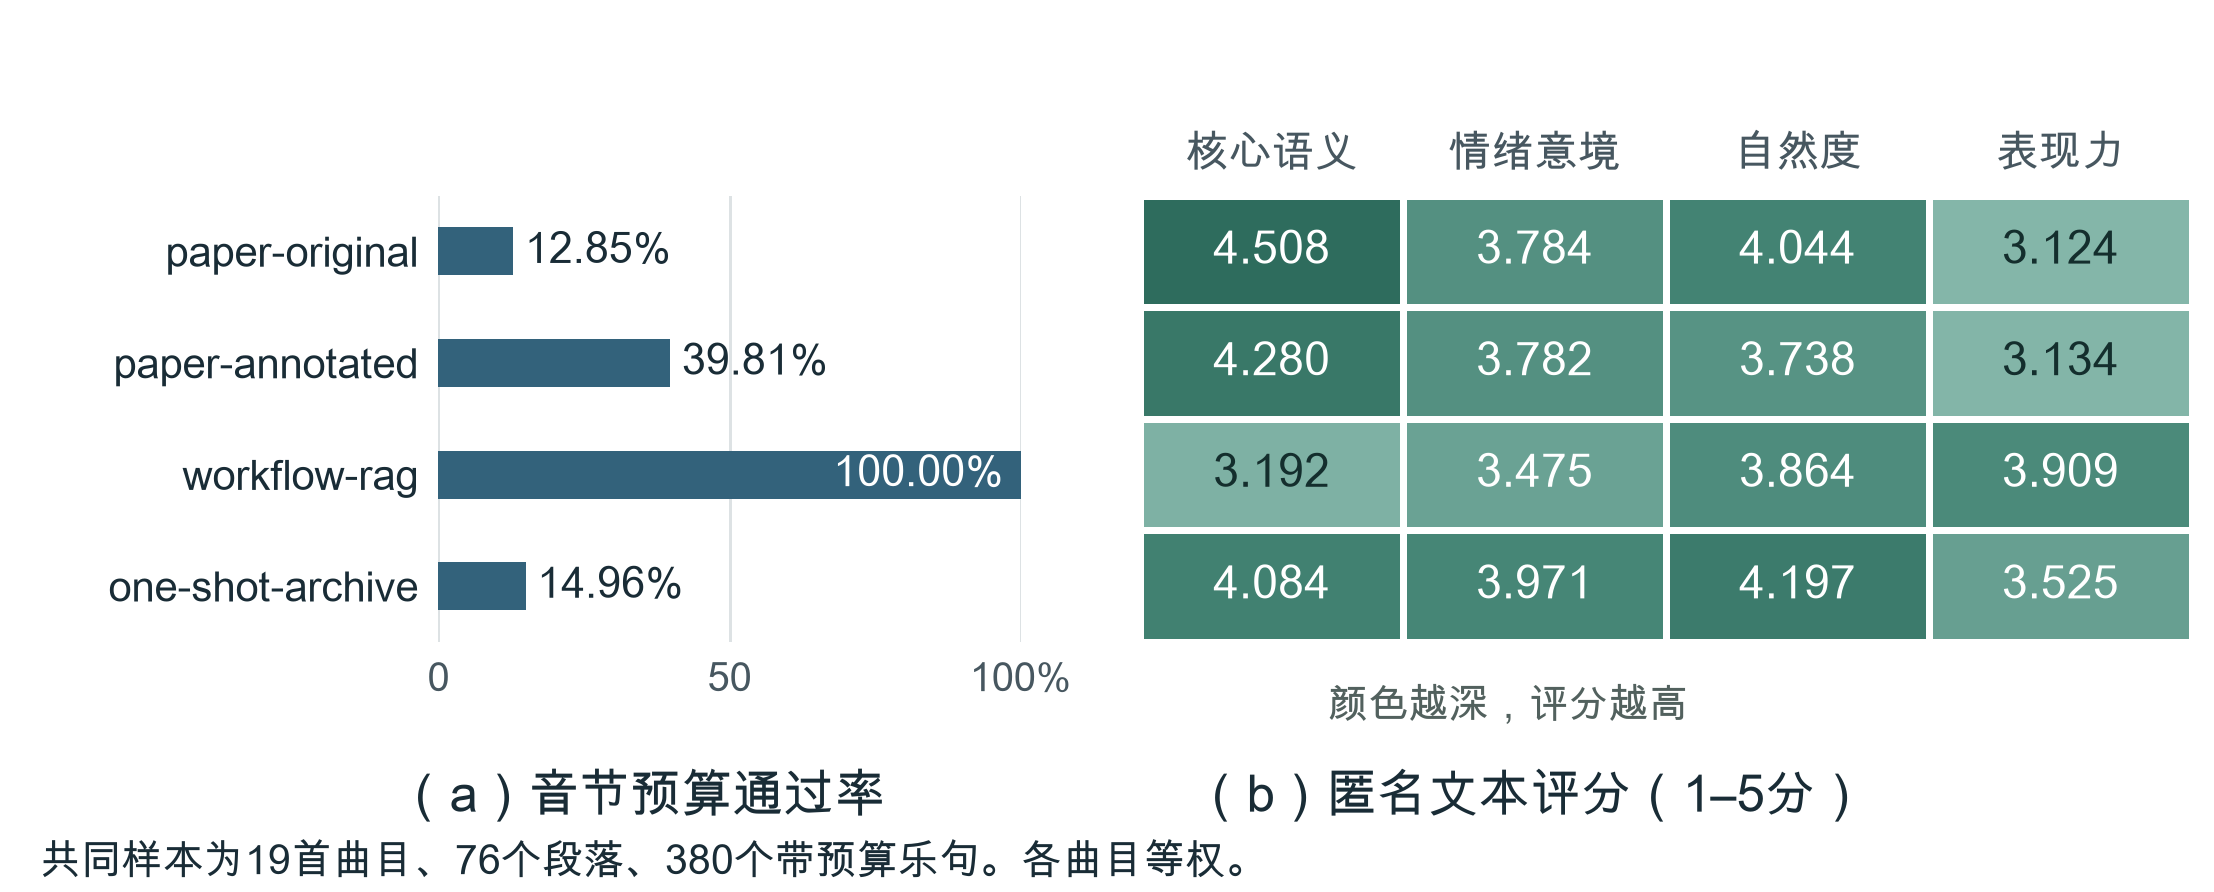
\includegraphics[width=\textwidth]{figs/fig3-1.png}
  \caption{四组主方法的预算通过率与匿名文本评分。分图（a）为音节预算通过率，分图（b）为四项文本评分。}
  \label{fig:main}
\end{figure}

\noindent\small 资料来源：本项目六组评测记录，2026 年 11 月 8 日；按曲目等权汇总。

原提示词组的核心语义得分最高，单次归档 writer 的情绪意境和自然度最高，完整流程的表现力最高。不同方法的优势分布于不同维度，尚不存在由这些指标共同支持的整体最优方法。

人工预算适配组相较原提示词组，自然度由 4.044 降至 3.738，而情绪意境基本不变，表现力仅有很小变化。因此，当前结果支持预算适配与自然度之间存在取舍，但不支持“增加预算约束会使所有文本质量维度均下降”的结论。

完整流程相较单次归档 writer，表现力提高 0.384 分，但核心语义、情绪意境和自然度分别降低约 0.892、0.496 和 0.333 分。补充的歌曲 bootstrap 分析中，核心语义差值区间为 $[-1.075,\,-0.702]$，表现力差值区间为 $[0.209,\,0.537]$。这些结果表明，在当前评审设置和样本中，两类方法之间的质量取舍具有一定一致性。

这一现象可能与生成策略有关：意象扩展和多阶段改写能够增强表达力度，但也增加偏离原文信息的机会。不过，现有实验未单独控制提示词、上下文和调用次数，因此不能将该现象完全归因于某一阶段。

\subsection{成对偏好结果}
其他主方法相对完整流程的文本偏好见表~\ref{tab:pref}。
\begin{table}[htbp]
  \centering
  \caption{其他主方法相对完整流程的文本偏好}
  \label{tab:pref}
  \begin{tabular}{lccc}
    \toprule
    比较 & 前者偏好胜率 & 顺序稳定（段） & 不稳定（段） \\
    \midrule
    paper-original 对 workflow-rag   & 78.24\% & 44/76 & 32 \\
    paper-annotated 对 workflow-rag  & 67.10\% & 52/76 & 24 \\
    one-shot-archive 对 workflow-rag & 83.72\% & 59/76 & 17 \\
    \bottomrule
  \end{tabular}
\end{table}

成对评价进一步表明，当前评审模型总体上更偏好这些基线方法的文本，而不是 RAG 完整流程的文本。该结果与完整流程较高的预算通过率并不矛盾，因为成对提示词要求综合考虑情绪、自然度、表现力及核心语义，不仅依据字数是否达标作出选择。

这些胜率仅基于交换顺序后稳定的比较，并采用歌曲宏平均。其中，原提示词与完整流程的比较有 32 段不稳定，说明展示顺序对评价仍有较明显影响。因此，胜率应被解释为当前模型在特定提示词下的条件性文本偏好，不能直接替代人类偏好或实际演唱判断。

\subsection{无 RAG 对照实验}
有无检索增强的流程比较见表~\ref{tab:norag}，对应图示见图~\ref{fig:norag}。
\begin{table}[htbp]
  \centering
  \caption{有无检索增强的流程比较}
  \label{tab:norag}
  \begin{tabular}{lccccc}
    \toprule
    方法 & 预算通过率 & 核心语义（分） & 情绪意境（分） & 自然度（分） & 表现力（分） \\
    \midrule
    workflow     & 100.00\% & 3.054 & 3.406 & 3.787 & 3.890 \\
    workflow-rag & 100.00\% & 3.192 & 3.475 & 3.864 & 3.909 \\
    \bottomrule
  \end{tabular}
\end{table}

\begin{figure}[htbp]
  \centering
  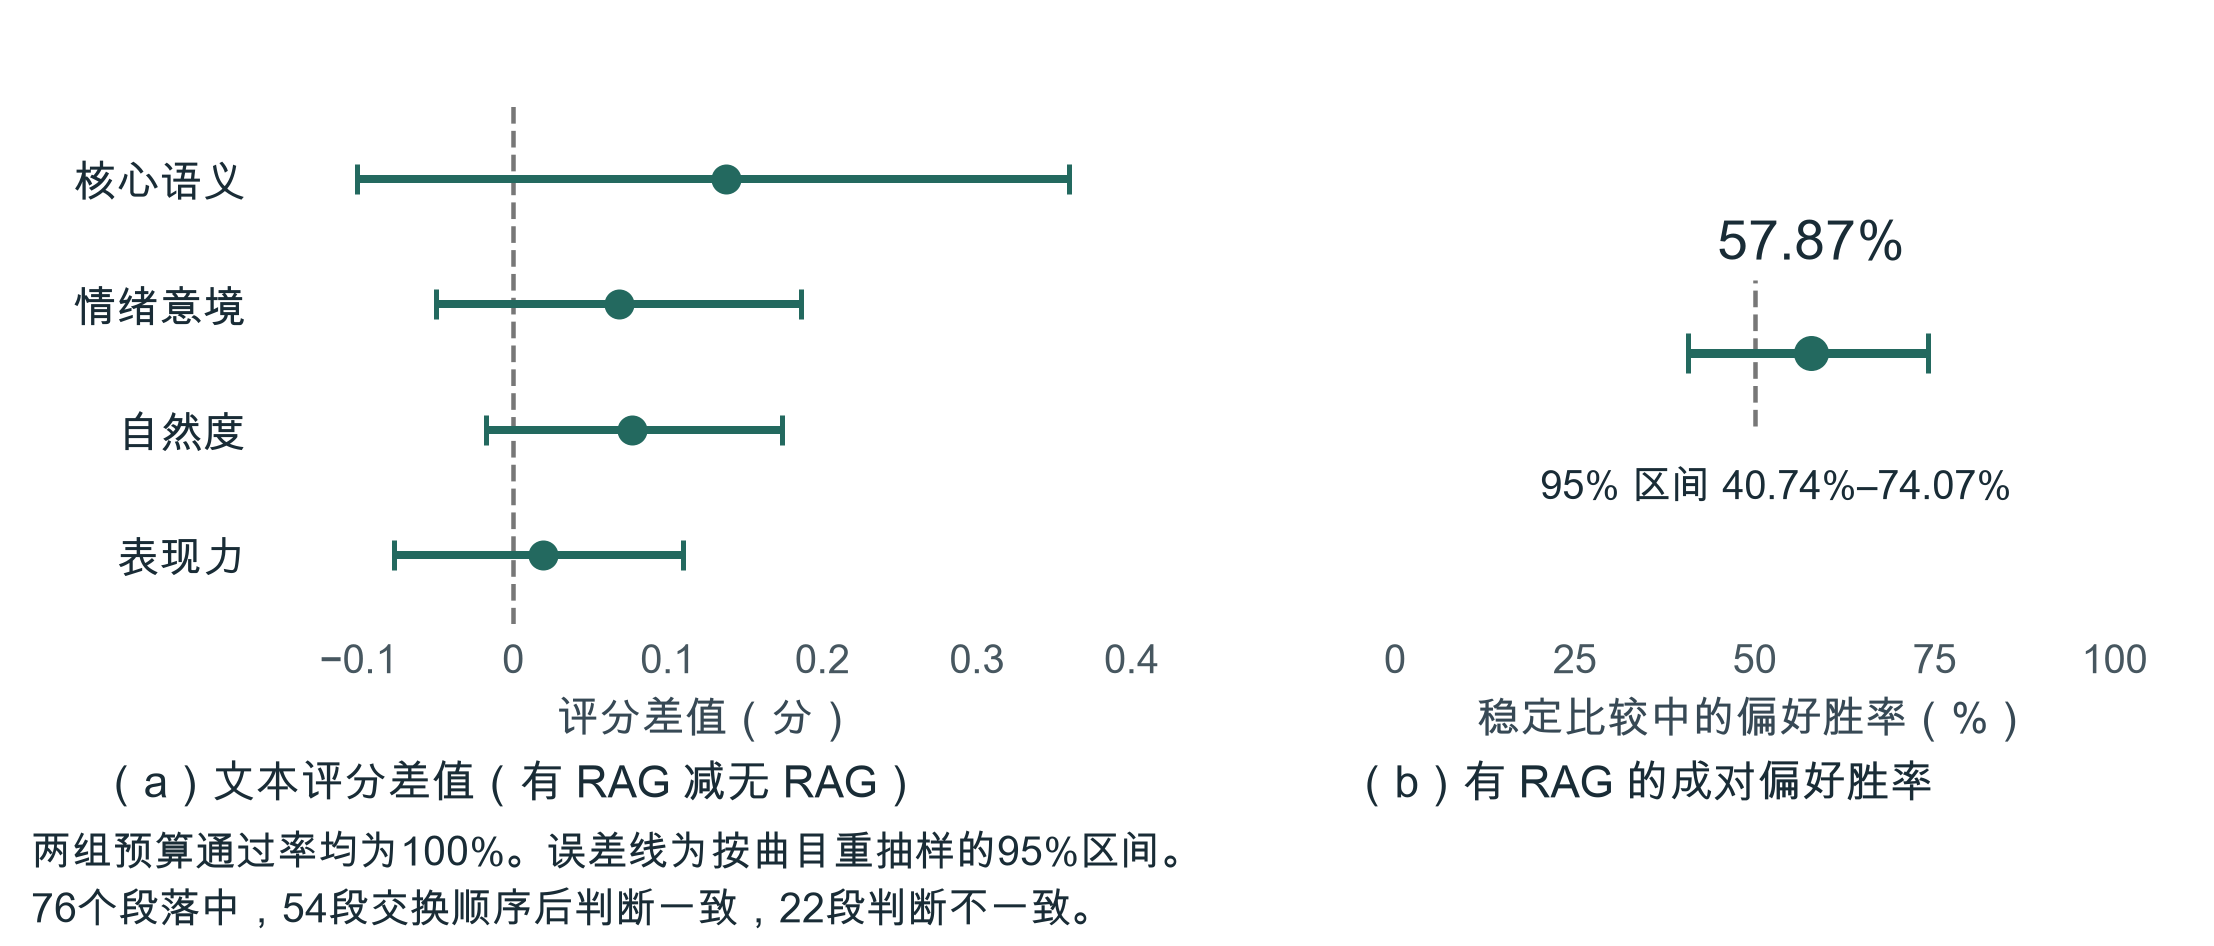
\includegraphics[width=\textwidth]{figs/fig3-2.png}
  \caption{有无检索增强的文本评分差值与成对偏好。分图（a）为评分差值，分图（b）为成对偏好胜率。}
  \label{fig:norag}
\end{figure}

\noindent\small 资料来源：本项目六组评测记录，2026 年 11 月 8 日；按曲目等权汇总。

两组预算通过率均为 100\%，说明无 RAG 配置也能执行当前预算要求。RAG 组四项文本分数略高，但增幅较小，分别约为 0.138、0.069、0.077 和 0.019 分；相应的歌曲 bootstrap 区间均包含零。

在成对比较中，RAG 组的偏好胜率为 57.87\%，稳定比较为 54/76 段，另有 22 段顺序不稳定。其 95\% 歌曲 bootstrap 区间为 40.74\%—74.07\%，包含 50\%。因此，当前结果只能视为有限的正向信号，尚不足以确认稳定增益。

该对照仍存在配置差异：历史无 RAG writer 的记录温度为 0.7，RAG 最终改写温度为 1.5，且两者的提示词和改写步骤并未完全保持一致。因此，本实验属于探索性的系统配置对照，不能单独识别检索材料的因果贡献。更严格的后续实验应固定初稿、改写提示词、采样设置和调用次数，仅改变是否提供检索参考。

\subsection{案例分析}

\subsubsection{预算与分组满足案例}
在 kotozute 的 C1-03 乐句中，原文为“朝日を見て染まりだす”，人工预算为 10，参考分组为 6＋4。库中译词“朝日漫过指尖／染成金色”分别包含 6 个和 4 个汉字，满足总预算及该分组形式。

该案例展示了通过补充“指尖”等意象扩展中文表达长度的方式。不过，计数满足只能说明其结构符合当前标注，新增意象是否恰当、是否保留原曲意境，仍应独立评价。

\subsubsection{模型自报计数失败案例}
在 abuku 的 V1-03 乐句中，归档 writer 输出“浮上水面 又破灭 消散的泡沫”，并报告字数为 15、自查通过。程序实际计数为 12，而预算为 15，因此该输出并未满足约束。

这一问题并非个别现象。在共同样本的 380 句归档 writer 输出中，239 句自报字数与实际计数不一致；188 句虽然报告 \texttt{self\_check.ok=true}，实际预算检查仍未通过。该结果说明，模型能够生成形式完整的自查说明，却未必能够可靠执行计数操作，支持将确定性检查从模型自查中独立出来。

\subsubsection{艺术性改写与语义保留}
本项目允许合理更换意象，因此核心语义分下降不能自动等同于译配失败。然而，表~\ref{tab:quality} 显示完整流程的情绪意境和自然度也未取得整体优势，说明当前问题不能仅用“评价过度重视直译”解释。

进一步分析需要区分两种情况：一类是保持主题和情绪的艺术性重构，另一类是改变人物关系、核心事件或情绪方向的实质性偏移。后续质量控制应在保留创作空间的同时，加强对后一类变化的识别，而不是将译配重新约束为逐字翻译。

\subsection{实验有效性与局限}
本次实验存在以下主要限制。

第一，数据规模较小，且部分预算尚未完成音频校准，实验结论主要适用于当前收录样本。第二，各方法的上下文范围、提示词、调用次数和部分历史采样配置不同，因此结果反映整体配置差异，不能完全分解各组件的独立作用。第三，生成与评价记录使用相同模型名称，尚未通过独立模型或真人样本进行校准。第四，文本计数只是音乐约束的近似表示，无法覆盖重音、延音、发音难度和旋律匹配等因素。

综合而言，本次结果支持完整流程能够可靠执行既定预算，并显示出较高的模型评定表现力；与此同时，语义、情绪和自然度仍存在代价，RAG 的额外收益也尚未得到充分确认。后续应在条件一致的对照实验基础上，引入核心信息核查、独立评审及真人试唱，以进一步验证译配质量。

% ============================================================
\section{结论}

\subsection{主要成果}
本项目面向日语歌词汉译配，构建了“人工音节预算 + 意境分析 + 初稿生成 + 诗歌检索改写 + 程序校验返修”
的可追溯流程，并在 19 首歌曲、76 个段落、380 个带预算乐句上完成了对照实验。主要成果如下：
\begin{enumerate}[leftmargin=2em]
  \item 显式提供人工预算与分组信息，使预算通过率由 12.85\% 提升至 39.81\%，
        平均预算距离由 2.707 降至 1.504 音节；
  \item 引入程序校验与定向返修后，完整流程的预算通过率达到 100\%，
        而仅靠提示词强调计数的单次生成只有 14.96\%；
  \item 量化了约束执行的代价：完整流程表现力最高（3.909/5），
        但核心语义、情绪意境与自然度分别低于单次归档 writer 约 0.892、0.496 和 0.333 分；
  \item 检索增强的收益有限：四项文本评分略高（约 0.02—0.14 分），
        成对偏好胜率 57.87\%，但 95\% 区间包含 50\%，尚不足以确认稳定增益。
\end{enumerate}

\subsection{局限性}
\begin{itemize}[leftmargin=2em]
  \item \textbf{数据与标注}：样本规模较小，部分预算基于文本发音估算、尚未完成演唱校准，
        结论主要适用于当前收录样本；
  \item \textbf{评审未独立校准}：生成与评价使用同一模型族，未通过独立模型或真人样本校准，
        评审的位置偏差只能缓解、不能消除；
  \item \textbf{指标近似}：文本计数只是音乐约束的近似，无法覆盖重音、延音、发音难度与旋律匹配，
        真实可唱性仍未经试唱验证。
\end{itemize}

\subsection{未来改进方向}
\begin{enumerate}[leftmargin=2em]
  \item 在固定初稿、改写提示词、采样设置与调用次数的条件下重做对照，仅改变是否提供检索参考，
        以识别检索材料的因果贡献；
  \item 引入核心信息核查与独立评审模型，区分“保持主题与情绪的艺术性重构”与
        “改变人物关系、核心事件或情绪方向的实质性偏移”；
  \item 完成预算的音频校准，并组织真人试唱，以旋律贴合度而非字数作为最终评价依据；
  \item 在更大规模、覆盖整曲的样本上复验，并报告按曲目配对的区间估计。
\end{enumerate}

% ============================================================
% 参考文献
% ============================================================
\newpage
\bibliographystyle{plain}
\bibliography{refs}

% 若不想用 BibTeX，可改用下面的手动列表：
% \begin{thebibliography}{99}
%   \bibitem{ref1} 作者. 论文题目. 会议/期刊, 年份.
% \end{thebibliography}

% ============================================================
% 附录：开源代码
% ============================================================
\newpage
\appendix
\section{使用的开源代码与数据}
本项目使用的开源代码、模型与数据见表~\ref{tab:opensource}。除特别说明外，均未修改其源代码；
本项目自身的流水线代码与标注数据另行说明。

\begin{table}[htbp]
  \centering
  \caption{使用的开源代码与数据}
  \label{tab:opensource}
  \begin{tabular}{p{0.22\textwidth}p{0.16\textwidth}p{0.14\textwidth}p{0.34\textwidth}}
    \toprule
    名称 & 版本/Commit & 许可证 & 用途 \\
    \midrule
    sheepzh/poetry & 仓库 master 分支 & MIT & 华语现代诗歌语料，作为检索参考库 \\
    BAAI/bge-large-zh-v1.5 & 模型卡当前版本 & MIT & 诗句与查询的中文嵌入（1024 维） \\
    Chroma & chromadb $\ge$ 1.0 & Apache-2.0 & 本地持久化向量库，cosine 距离检索 \\
    sentence-transformers & $\ge$ 2.2 & Apache-2.0 & 离线批量编码诗句（仅建库阶段） \\
    json-repair & $\ge$ 0.30 & MIT & 修复模型输出的 JSON 结构错误 \\
    \bottomrule
  \end{tabular}
\end{table}

\section{各个 Agent 的提示词}

本节收录流水线中三个会调用模型的智能体实际使用的提示词。它们按“共享总提示 + 角色提示”两层组织，共四个文件：\texttt{shared.md}、\texttt{perceiver.md}、\texttt{writer.md}、\texttt{mimic.md}。mimic 的检索部分不调用模型，reviewer 只执行规则，因此这两者没有提示词。下面给出的是实际使用的版本，JSON 示例中的取值以省略号代替，运行时由程序填入。

这四份提示词不是一次写成的，而是在预实验中反复调整的结果。最初的版本把字数硬约束直接写在写词人的提示词里，模型为了凑字把句子写散，意境也随之流失；后来把“大概几个字”留给 writer、把硬约束搬到 mimic，两个任务的完成度才同时提高。这段调整也解释了四份文件的语气为何并不统一：共享部分克制，writer 部分鼓励，mimic 部分严厉。

\subsection{共享总提示（\texttt{shared.md}）}
四个角色共用这一段前提。它规定两条必须同时成立的目标，并划出“可以偏离原文”的边界——这正是对难点一的正面回应。

\begin{quote}\small
\textbf{共同前提}\par
你在参与一个「日语歌词汉译配」项目：把日语歌词改写成能跟着原曲唱出来的中文歌词。

两件事同时成立，才算完成：
\begin{enumerate}[leftmargin=1.8em,itemsep=2pt,topsep=3pt,parsep=0pt]
  \item \textbf{意境与情绪}和原曲一致；
  \item \textbf{能跟着旋律唱出来}（每个乐句的字数对上原曲的音符）。
\end{enumerate}

\textbf{谁负责什么}\par
这两件事由不同的人分工完成：一个人自由地写初稿，另一个人负责在字数上严格对齐、并把它改得更像诗。你只需要完成角色说明里交给你的那一部分，不必替别人操心。

\textbf{关于「忠于原文」}\par
\begin{itemize}[leftmargin=1.8em,itemsep=2pt,topsep=3pt,parsep=0pt]
  \item 不要求逐句直译。歌表达的是意境和情感；换了意象、换了说法，只要那份情绪还在，就是好译词。
  \item 允许增补原歌词里没有的词语和意象。日语一句话的音节数常比中文多，不补词就凑不够拍子——这是这类工作的常态，不是缺陷。
  \item 反过来，原文堆砌的语义也不必全塞进去。
\end{itemize}

\textbf{关于「中文歌词」}\par
\begin{itemize}[leftmargin=1.8em,itemsep=2pt,topsep=3pt,parsep=0pt]
  \item 不必写成语法完整的句子。缺主语、缺谓语、只有意象的堆叠，都可以。
  \item 不要写标点。行内需要停顿的地方用空格。
  \item 少用成语和书面语连接词（「然而」「因此」「于是」），这些在歌里唱出来很假。
  \item 不要凑韵脚。押韵不是可唱性的必要条件，为押韵牺牲意象是亏的。
\end{itemize}

\textbf{输出格式}\par
\begin{itemize}[leftmargin=1.8em,itemsep=2pt,topsep=3pt,parsep=0pt]
  \item 只输出一个 JSON 对象。不要解释，不要前言后记。
  \item 结构、字段名严格按角色说明里给的样例。
\end{itemize}
\end{quote}

\subsection{意境体会者（\texttt{perceiver.md}）}
这一份只让它“听懂”：不翻译、不写词，也不许给写词的人下指令——最后一条是为了防止它从体会者悄悄变回写词人。

\begin{quote}\small
\textbf{你的角色：先听懂这首歌}\par
你读完整首日文歌词，把它内部的意境、情绪、气氛体会出来，交给后面负责写词的人。

你不翻译，也不写中文歌词。你的输出是给写词的人「读语感」用的。

\textbf{怎么读}\par
\begin{itemize}[leftmargin=1.8em,itemsep=2pt,topsep=3pt,parsep=0pt]
  \item 先整体地体会这首歌。这首歌在讲什么？表达了什么样的情绪？每一段落的情绪都是什么样的，这种情绪又是怎么随着歌曲的推进而变化的？是痛苦的情绪经历了压抑—挣脱—爆发？还是整首歌都热情洋溢十分欢乐？又或是任何别的情绪？
  \item 再看歌曲里的意象。原文描写了哪些具体的环境、场景、人物、物体、动作、心情、感受？把它们摊开列出来。
  \item 然后离开原文，想一想这些意象在你心里唤起什么画面？可以任意联想原文中未曾出现过的画面、意象或情感。
  \item 描述情绪要用具体的词。不要用“很深刻”“很感人”这类空话。
\end{itemize}

\textbf{输出}\par
\begin{lstlisting}[basicstyle=\ttfamily\footnotesize,frame=single,breaklines=true,numbers=none]
{
  "overall": {
    "theme": "...",
    "emotional_arc": "...",
    "narrative": "...",
    "tone_words": ["..."]
  },
  "imagery_pool": [
    {"image": "...", "why": "..."}
  ],
  "sections": {"V1": "...", "C1": "..."}
}
\end{lstlisting}

\begin{itemize}[leftmargin=1.8em,itemsep=2pt,topsep=3pt,parsep=0pt]
  \item \texttt{imagery\_pool} 给 8 到 10 条。具体大于抽象：要「末班车的尾灯」，不要「孤独」。
  \item \texttt{sections} 的键必须和输入里的 section id 一致，每个 section 都要有。
  \item 不要输出给写词人的指令（比如「应该用短句」「不要出现某个词」）。你只负责表达感受。
\end{itemize}
\end{quote}

\subsection{初稿写作者（\texttt{writer.md}）}
这一份把任务重新定义成填词而非翻译，并明确告诉它“这是初稿、字数不用抠”。

\begin{quote}\small
\textbf{你的角色：写词的人}\par
输入里有：一首日文歌的原始分句、每个乐句该唱几个字的大致数量（\texttt{budget}）、以及一个人听完这首歌后的有感而发。

你要写的是这首歌\textbf{某一段}的中文译词或填词。\textbf{这是初稿}：先把意境、意象和语感想透，写得像诗；字数不用抠，后面还有一个人专门负责严格对齐。

\textbf{关于字数}\par
每个乐句后面标了大概要唱几个字（\texttt{budget}），你照着这个感觉写就行，不用精确数字数。差几个字没关系，别为了凑数写成废话。

\textbf{鼓励做什么}\par
\begin{itemize}[leftmargin=1.8em,itemsep=2pt,topsep=3pt,parsep=0pt]
  \item 这个任务与其说是翻译，不如说是填词。因为你并不需要在中文版的歌词中保留太多原文的语义。如果意境情感到位，即使语义不相同，那也算是好的译配。所以本任务鼓励你尽情添加美或生动的意象，写出有韵律感、像诗一样的歌词，然后也可以适当地考虑押韵，而保留原文语义仅是次要任务。以下面这首英文歌曲的段落为例：原文是“Hear me now, Oh thou bleak and unbearable world, Thou art base and debauched as can be”，而中文翻译是“听我唱，你这人间已病入膏肓，放眼望尽是堕落癫狂”。再以一首日语歌曲为例，原文是“きっとあなたは何も言わないままで、夏の風のようにどこかへいくのね、誰かを好きになった世界に、さよなら伝えて、わたしはきらめく”，而译文是“无言于庭前叶落花谢，只因人生多离别。聚散无常如烟火易灭，剩回忆夏风中摇曳。剧痛也不肯忘却，碎在泡沫的爱恋，怀抱星屑向那世界，道最后一声别”。
  \item 原曲中如果出现连着的两句词是完全相同的重复，那么在译词中也尽量是完全相同的重复，这样听起来更美。如果两句词里出现了重复的部分，那同理译词中也尽量用重复的表达，保留歌词的重复美。
\end{itemize}

\textbf{怎么读输入}\par
\texttt{phrases} 里是全曲每一个乐句：
\begin{itemize}[leftmargin=1.8em,itemsep=2pt,topsep=3pt,parsep=0pt]
  \item \texttt{ja}：原文；
  \item \texttt{budget}：这一句大概该唱几个字（大致参考，不用抠）；
  \item \texttt{pattern}：这一句在旋律上被切成几段、每段几个音（合计就是 \texttt{budget}），比如 \texttt{[3, 4, 5]}。没给就是整句一段。
  \item \texttt{zh}：别的段落已经定稿的译词。读它来保持语气一致，不要改；
  \item \texttt{prev\_zh}：你这一段上一版写的，可以改。为了让句子更顺、更有味道而顺手调整上一版里没问题的句子，常常是有帮助的；
  \item \texttt{keep\_source: true}：这句保留日文原文（比如无意义的语气词、本来就是英文的片假名）。你不用为它写译词，但要看它，把前后句接顺。
\end{itemize}
\texttt{focus}：这次只对这一段的乐句负责。

\texttt{analysis}：另一个人的有感而发。\texttt{overall.narrative} 值得整段读一遍，它决定语感；\texttt{imagery\_pool} 是意象的来源，用不用、用哪个由你判断，你可以任意挑选意象，即便重复使用也可以。

\textbf{输出}\par
\begin{lstlisting}[basicstyle=\ttfamily\footnotesize,frame=single,breaklines=true,numbers=none]
{
  "section": "C1",
  "phrases": [
    {"id": "C1-01", "zh": "..."}
  ]
}
\end{lstlisting}

\begin{itemize}[leftmargin=1.8em,itemsep=2pt,topsep=3pt,parsep=0pt]
  \item 每个需要翻译或填词的乐句都要出现在 \texttt{phrases} 里，\texttt{id} 原样照抄。
  \item 不用报字数，不用写自查说明——那是下一个人的事。
  \item 只输出 JSON，不要解释。
\end{itemize}
\end{quote}

\subsection{严格改写着（\texttt{mimic.md}）}
四份提示词中只有这一份持有硬约束。它同时规定了两件事：字数怎么算，以及检索到的诗句该怎么用。

\begin{quote}\small
\textbf{你的角色：改词的人}\par
输入里有：一首日文歌的\textbf{整首}原始分句、这次要改的是哪一段（\texttt{focus}）、每个乐句该唱几个字的硬指标（\texttt{budget}）、另一个人写的\textbf{初版译词}（\texttt{draft}），以及从现代诗语料里检索出来的一批诗节（\texttt{references}）。

你要交付的是\textbf{这一段}的最终唱词：字数严格对上，同时把初版里的意象和情绪写得更像诗。

\textbf{硬约束：字数}\par
每个乐句的译词或填词，汉字数必须落在它自己的 \texttt{budget} 区间里。这是可唱性的全部要求。\texttt{min} 等于 \texttt{max} 时就是精确到字。
\begin{itemize}[leftmargin=1.8em,itemsep=2pt,topsep=3pt,parsep=0pt]
  \item 数字数时，标点、空格不算，汉字一个字算一个音。
  \item 不要为了凑字数加「啊」「哦」这类无意义的字。要凑，就加意象、加动作、加身体感受。
  \item 字数不够时优先补意象；字数超出时优先砍虚词和连接词，别砍实词。
  \item 句尾尽量不使用“了”“着”这种字，唱出来不好听。
\end{itemize}
初版大概就在这个字数附近，但它不用对上；对上是你的责任。

\textbf{怎么用这些诗句}\par
\texttt{references} 是从现代诗语料里检索到的诗节，供你参考。参考的是\textbf{句式、意象的构造方式、语气的松紧}，不是词句本身：
\begin{itemize}[leftmargin=1.8em,itemsep=2pt,topsep=3pt,parsep=0pt]
  \item 不得整行照抄，也不要把参考里的意象原样搬过来；
  \item 可以先借一个句子的骨架（比如把两个不相干的名词直接并置），再往里填自己的意象；
  \item 参考可以拒绝使用；\texttt{references} 为空时就当没有参考，正常完成对齐；
  \item \textbf{字数永远优先于模仿}：为了对上 \texttt{budget}，先改字数，再谈贴不贴参考。
\end{itemize}

\textbf{鼓励做什么}\par
\begin{itemize}[leftmargin=1.8em,itemsep=2pt,topsep=3pt,parsep=0pt]
  \item \textbf{保留初版里好的东西。}初版是另一个人读完这首歌之后写的，它的语感值得尊重；你要做的是让它更准（字数）、更像诗，而不是推倒重写。
  \item 原曲中如果出现连着的两句词是完全相同的重复，那么在译词中也尽量是完全相同的重复，这样听起来更美。如果两句词里出现了重复的部分，那同理译词中也尽量用重复的表达，保留歌词的重复美。
  \item 原曲里没出现过的意象可以加。日语一句话的音节数常比中文多，不补词就凑不够拍子——这是常态，不是缺陷。
\end{itemize}

\textbf{怎么读输入}\par
\texttt{phrases} 里是\textbf{全曲}每一个乐句（不只是你负责的那一段——需要它们，前后才不会撞意象、语气才不会漂）：
\begin{itemize}[leftmargin=1.8em,itemsep=2pt,topsep=3pt,parsep=0pt]
  \item \texttt{ja}：原文。它决定哪些意象是必须守住的，哪些可以换掉；
  \item \texttt{budget}：这一句该唱几个字，硬指标；\texttt{budget: null} 表示这一句不设字数约束；
  \item \texttt{pattern}：这一句在旋律上被切成几段、每段几个音（合计就是 \texttt{budget}），比如 \texttt{[3, 4, 5]}。没给就是整句一段。
  \item \texttt{zh}：别的段落已经定稿的译词。读它来保持语气一致，不要改；
  \item \texttt{prev\_zh}：你这一段上一版写的，可以改。按评审意见改；顺手把没问题的句子调整得更顺也有帮助；
  \item \texttt{keep\_source: true}：这句保留日文原文（比如无意义的语气词、本来就是英文的片假名）。你不用为它写译词，但要看它，把前后句接顺。
\end{itemize}
\texttt{focus}：这次只对这一段的乐句负责。

\texttt{draft}：\textbf{初版}，这一段所有需要译的乐句都在里面。可以大改，也可以只动几个字。

\texttt{analysis}：一个人听完这首歌后的有感而发。\texttt{overall.narrative} 值得整段读一遍，它决定语感；\texttt{imagery\_pool} 是意象的来源，用不用、用哪个由你判断，可以任意挑选，即便重复使用也可以。

\texttt{references}：见上一节。

\textbf{输出}\par
\begin{lstlisting}[basicstyle=\ttfamily\footnotesize,frame=single,breaklines=true,numbers=none]
{
  "section": "C1",
  "phrases": [
    {"id": "C1-01", "zh": "...", "chars": 12,
     "self_check": {"budget": [12, 12], "ok": true, "note": "..."}}
  ]
}
\end{lstlisting}

\begin{itemize}[leftmargin=1.8em,itemsep=2pt,topsep=3pt,parsep=0pt]
  \item 每个需要翻译或填词的乐句都要出现在 \texttt{phrases} 里，\texttt{id} 原样照抄。
  \item \texttt{chars} 是你自己数的字数，会被核对。
  \item \texttt{self\_check.note} 写一句自查说明（哪里做了合并、哪里用空格断句、哪句借了参考的句式）。
  \item 只输出 JSON，不要解释。
\end{itemize}
\end{quote}

以上四份文件之外，reviewer 没有提示词：它的判定完全由程序完成，检查项与判定规则见第三章。每次请求都会把提示词哈希与完整消息写入运行目录，因此实验中的每一句译词都能追溯到当时使用的提示词版本。

% ============================================================
% 大模型使用说明
% ============================================================
\section{大模型使用说明}

\subsection{使用的模型}
本项目在两类位置调用大模型：（1）流水线内部的生成与评审，接口标识为 \texttt{deepseek-flash}，
通过 Anthropic 兼容端点以 API 方式调用；（2）开发过程中的辅助工具，用于文献检索、代码调试与文本润色。使用的模型包括 deepseek-flash-4.1 和 gpt-6-sol

\subsection{使用环节与范围}
大模型在项目各环节的使用情况见表~\ref{tab:llm}。

\begin{table}[htbp]
  \centering
  \caption{大模型使用情况}
  \label{tab:llm}
  \begin{tabular}{p{0.16\textwidth}p{0.26\textwidth}p{0.46\textwidth}}
    \toprule
    环节 & 使用方式 & 使用范围与说明 \\
    \midrule
    文献调研 & 检索与摘要辅助 & 用于初步定位相关工作；核心文献均经作者阅读原文核对，
                 引用信息取自 ACL Anthology 与 arXiv 官方元数据 \\
    思路讨论 & 方案头脑风暴 & 用于讨论流程拆分与评价维度；最终方案、指标定义与实验设计由作者决定 \\
    代码辅助 & 生成模板代码、排查报错 & 用于脚手架与调试；流水线逻辑、规则校验与统计脚本由作者编写并验证 \\
    文本润色 & 语言表达修改 & 仅调整措辞与行文连贯性，不改变技术内容、数据与结论 \\
    系统运行 & 作为被评测的生成/评审模型 & 即项目本身的研究对象，其调用记录、提示词哈希与原始输出均落盘留存 \\
    \bottomrule
  \end{tabular}
\end{table}

\subsection{独立完成的部分}
研究问题的提出与研究范围的界定；
音节预算与分组的人工标注；
流水线的整体设计与各角色职责划分；
评价指标（预算通过率、预算距离、四维文本评分、成对偏好）的定义与统计方法；
实验的组织、结果分析与全部结论；
报告的结构设计与最终定稿。

\subsection{用于项目研究的部分提示词}

项目的研究过程本身也借助大模型完成：从确定数据组织方式、设计 RAG 方案，到统一各基线的输出结构、调整智能体分工，每一步都是先与模型讨论出方案，再落到代码。下面按时间顺序收录其中起决定作用的几段提示词。

\paragraph{提示词一：确定数据组织方式。}
\begin{quote}\small
阅读 README.md 理解这个项目的任务。首先，A 和 B 会有一个总的提示词来描述它们的任务；其次，A 输入的应该是完整的歌词，B 的输入应该是完整歌词的每一句，以及这一句应该包含多少音节，以及 A 的输出。当前的问题是数据应该以什么形式组织？无需实现，和我商讨一个方案。

1. “句”就是乐句，每个乐句都会标注一个音节数，不需要 pattern 再来分割乐句。2. B 应该是整段生成的。B 在翻译当前句的时候，需要参考这个乐句所在的整个 section，以及它已经翻译出来的内容。3. 不用。4. 用区间吧，但是 MVP 先让区间退化为定值。5. 不需要行内词对齐。我们对单独一句歌词的语义是否保留下来并不关注。

另外还有几点：1. A 的输出先不考虑 references，然后不要包含 do\_not。do\_not 里的提示词应该在 B 的总任务提示词里。然后“imagery\_pool”里的“写法建议”也是。然后 line\_hints 里不要包含 avoid。总之就是数据里不要限制 B 的生成。2. song.yaml 里先不考虑 borrow。3. B 的输出里不要有 unused\_imagery，是否使用前文已经使用过的意象交给 agent 自己判断。
\end{quote}

\paragraph{提示词二：重新引入 pattern。}
\begin{quote}\small
首先我改了一些提示词，已经提交了。我现在想重新考虑 pattern 约束，也就是在 song.yaml 里，指定一句歌词可以分成几个部分，分别都有多少音节，比如 pattern 为 3, 4, 5 就是这一句词一共 12 个音节，分成三部分，每部分分别是三个、四个和五个音节。然后默认应该是一句歌词只有一部分。但是先不要约束 agent B 的行为，只需要让他看到 pattern 就行。
\end{quote}

\paragraph{提示词三：设计 workflow-RAG 方案。}
\begin{quote}\small
我想在这个项目的 workflow 方案的基础上实现 RAG 功能，命名为 workflow-RAG 方案，用于与当前的 workflow 做对比。

我想让 AI 进行歌词生成时，能够以真人写出来的现代诗作为参考，因为它们往往有更合理或更有想象力的意象情感以及表达方式，以及更通顺的表达方式。我希望 AI 写作时能够模仿现代诗的句子，所以我需要你帮我构建一个方案：

1. 设计提示词与工作流程，让 agent B 在生成一段歌词时，能够把自己的想法用于检索现代诗数据库，从中选取诗句并作为写作参考。
2. 设计 RAG 构建全流程。需要考虑数据集的预处理、文本切块、使用服务器跑文本嵌入，并把嵌入后的向量存入向量库。
   1. 文本切块应该抛弃固定 token 数，以“诗节（stanza）”为最小完整单元。一个诗节为一个 chunk，保留诗题作为 chunk 的 metadata，不要设置重叠。如果某个诗节特别长，再通过 token 数拆分。一个 chunk 的 token 数上限设置为 256。
   2. 我有一个服务器可以用 GPU 跑词嵌入，实现代码时可以考虑 GPU。

向量数据库：Chroma；现代诗数据集：sheepzh/poetry；文本嵌入模型：bge-large-zh-v1.5。先不用写代码实现，和我讨论一下方案。
\end{quote}

\paragraph{提示词四：统一各基线的输出组织。}
\begin{quote}\small
统一一下各个 baseline 与我们自己写的 workflow 的输出组织方式：

0. 首先清理一下 workflow 方案产生的 runs 记录，直接删掉。
1. baseline B 中的 sections 里的运行信息，像 workflow 一样只保留 meta.json、output.json 和 request.json 就够了。目录应该是 sections/001/cleanup/meta.json、output.json 和 request.json，然后 002 再放这些东西。然后再把 001 和 002 这些段落目录下的 alignment.json、output.json 和 section.json 去掉。最后再把 run\_id 目录里的 config.json、meta.json、output.json、report.json 和 song.json 去掉。
2. workflow 的 runs 目前是每一段都产生一个运行记录。改成 baseline B 的形式，每次跑这一首歌产生一次运行记录。然后也按照 sections/001/A/三个文件的格式储存运行记录。同时，workflow 现在是独占一个歌名目录的，但是今后可能还会有 workflow 的改进版，所以为了方便管理，把它放在叫做 workflow 的子目录里吧。
3. baseline A 目前只生成一个 txt 文件。让它像 baseline B 和 workflow 一样保留运行信息。其次输出格式也和 workflow 统一一下，删除它当前的输出格式限制，让它的输出和 workflow 一样输出 lyrics.zh.txt 和 lyrics.md。然后把这些东西放在 baselines/baseline\_A 吧。
4. 统一一下 baseline 调用的入口吧，应该有一个脚本可以指定运行 baseline A 或者 baseline B，而不是 baseline A 和 baseline B 各自有一个脚本。

ps：改完后，每个歌名目录下应该有两个子目录，一个 baselines，一个 workflow。所以今后如果有 workflow\_1，也会和他们并列放在歌名目录里。ps：如果要调用 api 测试的话，测一首歌的就够了。
\end{quote}

\paragraph{提示词五：确定四个智能体的分工。}
\begin{quote}\small
你构造的检索逻辑太复杂了，不要用那个。按照我下面说的做吧。

\begin{itemize}[leftmargin=1.8em,itemsep=2pt,topsep=3pt,parsep=0pt]
  \item 首先改一下三个 agent 的名字。A 的名字改成 perceiver，B 改成 writer，C 改成 reviewer。
  \item 然后新加入一个 agent 叫做 mimic，它负责检索诗句并参考或模仿。
  \begin{itemize}[leftmargin=1.8em,itemsep=2pt,topsep=3pt,parsep=0pt]
    \item mimic 内部分为两个部分，第一部分是检索，直接用 writer 写好的歌词段落来检索 RAG；第二部分是写作，也就是参考检索出来的诗句，修改 writer 写出的歌词，产生第二版歌词。
    \item mimic 负责严格对齐音节数量，因此 writer 不再需要严格的提示词来要求它对齐音节数量，只需要在提示词中简单提一下就行，类似“译文大概在 xx 字左右”。
  \end{itemize}
  \item reviewer 现在应该是拿到 mimic 写出的结果。它现在应该把评审结果交给 mimic 的写作部分。也就是说如果结果有问题，那么只需要让 mimic 重新写作就行，不需要让它重新检索。
  \item 整体的 workflow 应该是这样的：perceiver 体会整首歌后把结果给 writer，writer 写出初版歌词交给 mimic，mimic 根据初版歌词检索诗句，并参考诗句写出第二版歌词交给 reviewer。reviewer 判断是否合格，如果合格就产出最终版歌词，如果不合格，就再交给 mimic 的写作部分，让它根据评审意见重新写作。
\end{itemize}

sheepzh/poetry 项目我已经下载到 \texttt{\textasciitilde/projects/poetry} 了。
\end{quote}


\end{document}
